\section{Introduction}
\label{sec:intro}

Direct equation discovery continues to represent a key challenge and area of progress in scientific machine learning.
From a model selection perspective, it is important to guard against overfitting, since this compromises its ability to generalise and provide reliable forecasts. At the same time, we also want to enhance the interpretability and parsimony of the model. Thus, it is crucial to balance accuracy with interpretability and parsimony. These principles align with Occam’s razor, which states that among competing hypotheses that explain the data, the simplest one consistent with the observations should be preferred. 
The motivation is twofold: aesthetically, mathematically elegant theories are often considered more likely to be correct; empirically, simpler models tend to make more precise predictions, whereas complex models require more assumptions and are prone to overfitting (see \cite{mackay2003}). The Bayesian evidence and sparse identification of nonlinear dynamics (SINDy) are regarded as principled methods for model selection across statistics, machine learning, and the natural sciences because they naturally embody the principle of Occam’s razor.


Bayesian evidence provides a principled framework for implementing Occam's razor, with its theoretical foundation laid by David MacKay and Stephen Gull.
\cite{mackay1992} showed that the evidence integral $Z = \int P(\text{data} \mid \theta)\, P(\theta)\, \mathrm{d}\theta$
can be decomposed into a likelihood term measuring goodness-of-fit and an Occam factor that penalises unnecessary model complexity. This penalty enforces parsimony by down-weighting parameter dimensions that are not effectively constrained by the data, thereby discouraging overfitting. 
In parallel, \cite{gull1988} provided an information-theoretic justification for prior specification via the Maximum Entropy Principle, emphasising how the choice of prior encodes assumptions about model simplicity. This perspective later motivated the use of sparsity-inducing priors, such as the Laplace distribution \citep{park2008} and spike-and-slab formulations \citep{mitchell1988, george1993}, which concentrate probability mass near zero and thereby favour models where only a small subset of parameters are active.
The practical computation of Bayesian evidence has stimulated the development of specialised numerical methods. Nested Sampling \citep{buchner2016,buchner2023} and Thermodynamic Integration (TI) \citep{aponte2022} are among the most widely used algorithms for evaluating the evidence integral, with the former based on stochastic exploration of constrained likelihood contours and the latter grounded in statistical physics and particularly popular in cognitive and neurodynamical modelling. The Laplace approximation \citep{mackay2003} provides a computationally efficient alternative by performing a local quadratic expansion around the maximum a posteriori (MAP) estimate, though at the cost of reduced accuracy when the posterior is highly non-Gaussian. 
Building on these theoretical and computational advances, a large body of work (see, e.g., \cite{rougier2021, bayarri2012}) demonstrates that the marginal likelihood, or evidence, automatically balances data fit with model complexity, thereby embodying Occam’s razor without the need for ad-hoc penalisation. More recent contributions \citep{lotfi2022, knuth2015} further highlight both the strengths and limitations of evidence-based model comparison, particularly in high-dimensional and data-scarce regimes. Together, these studies establish Bayesian evidence as not only a theoretical embodiment of Occam’s razor but also a practical criterion for selecting parsimonious models that generalise well.


SINDy’s Sequentially Thresholded Least Squares (STLSQ) algorithm provides another useful framework for addressing the issue of overfitting in model selection. SINDy essentially reformulates equation discovery into a sparse dictionary learning framework, which can be used for model selection. 
It first generates a library containing all possible candidate functions of the data, and subsequently employs sparse regression to identify the functions that meaningfully represent the underlying dynamics, filtering out the superfluous ones. By enforcing parsimony through sparsity, SINDy yields interpretable models that strike a balance between accuracy and generalizability, while its streamlined structure also enables comparatively efficient and rapid learning relative to many other machine learning approaches.
SINDy has progressed markedly in recent years. Researchers have proposed a series of new algorithms, such as uncertainty quantification SINDy (UQ-SINDy), developed by \cite{hirsh2022}. They used MCMC and sparsifying priors; Ensemble-SINDy (E-SINDy), proposed by \cite{fasel2022}, which used the idea of bootstrap aggregating; and a rapid Bayesian identification framework constructed by \cite{fung2024} to address problems with scarce and noisy data. 


However, in computing the likelihood and posterior distribution, the current method is challenged by how uncertainty exists in both the dependent and independent variables. Since the principle of SINDy is to regress the derivatives of the time series against the time series itself, when there is uncertainty in the time series, it propagates through both the dependent and independent variables in the regression process. This setting, in which measurement noise affects both the predictors and the response, is known as the errors-in-variables (EIV) problem. 
However, despite the growing maturity of Bayesian SINDy methods, they are almost all built upon a common, standard regression assumption: that the model primarily accounts for noise in the dependent variable (the time derivative $\dot{x} $), while ignoring the fact that the state variables $x$, which serve as the independent variables, are themselves inevitably derived from noisy measurements. This violates a fundamental premise of regression analysis and may lead to systematic bias in model selection.


\begin{figure}
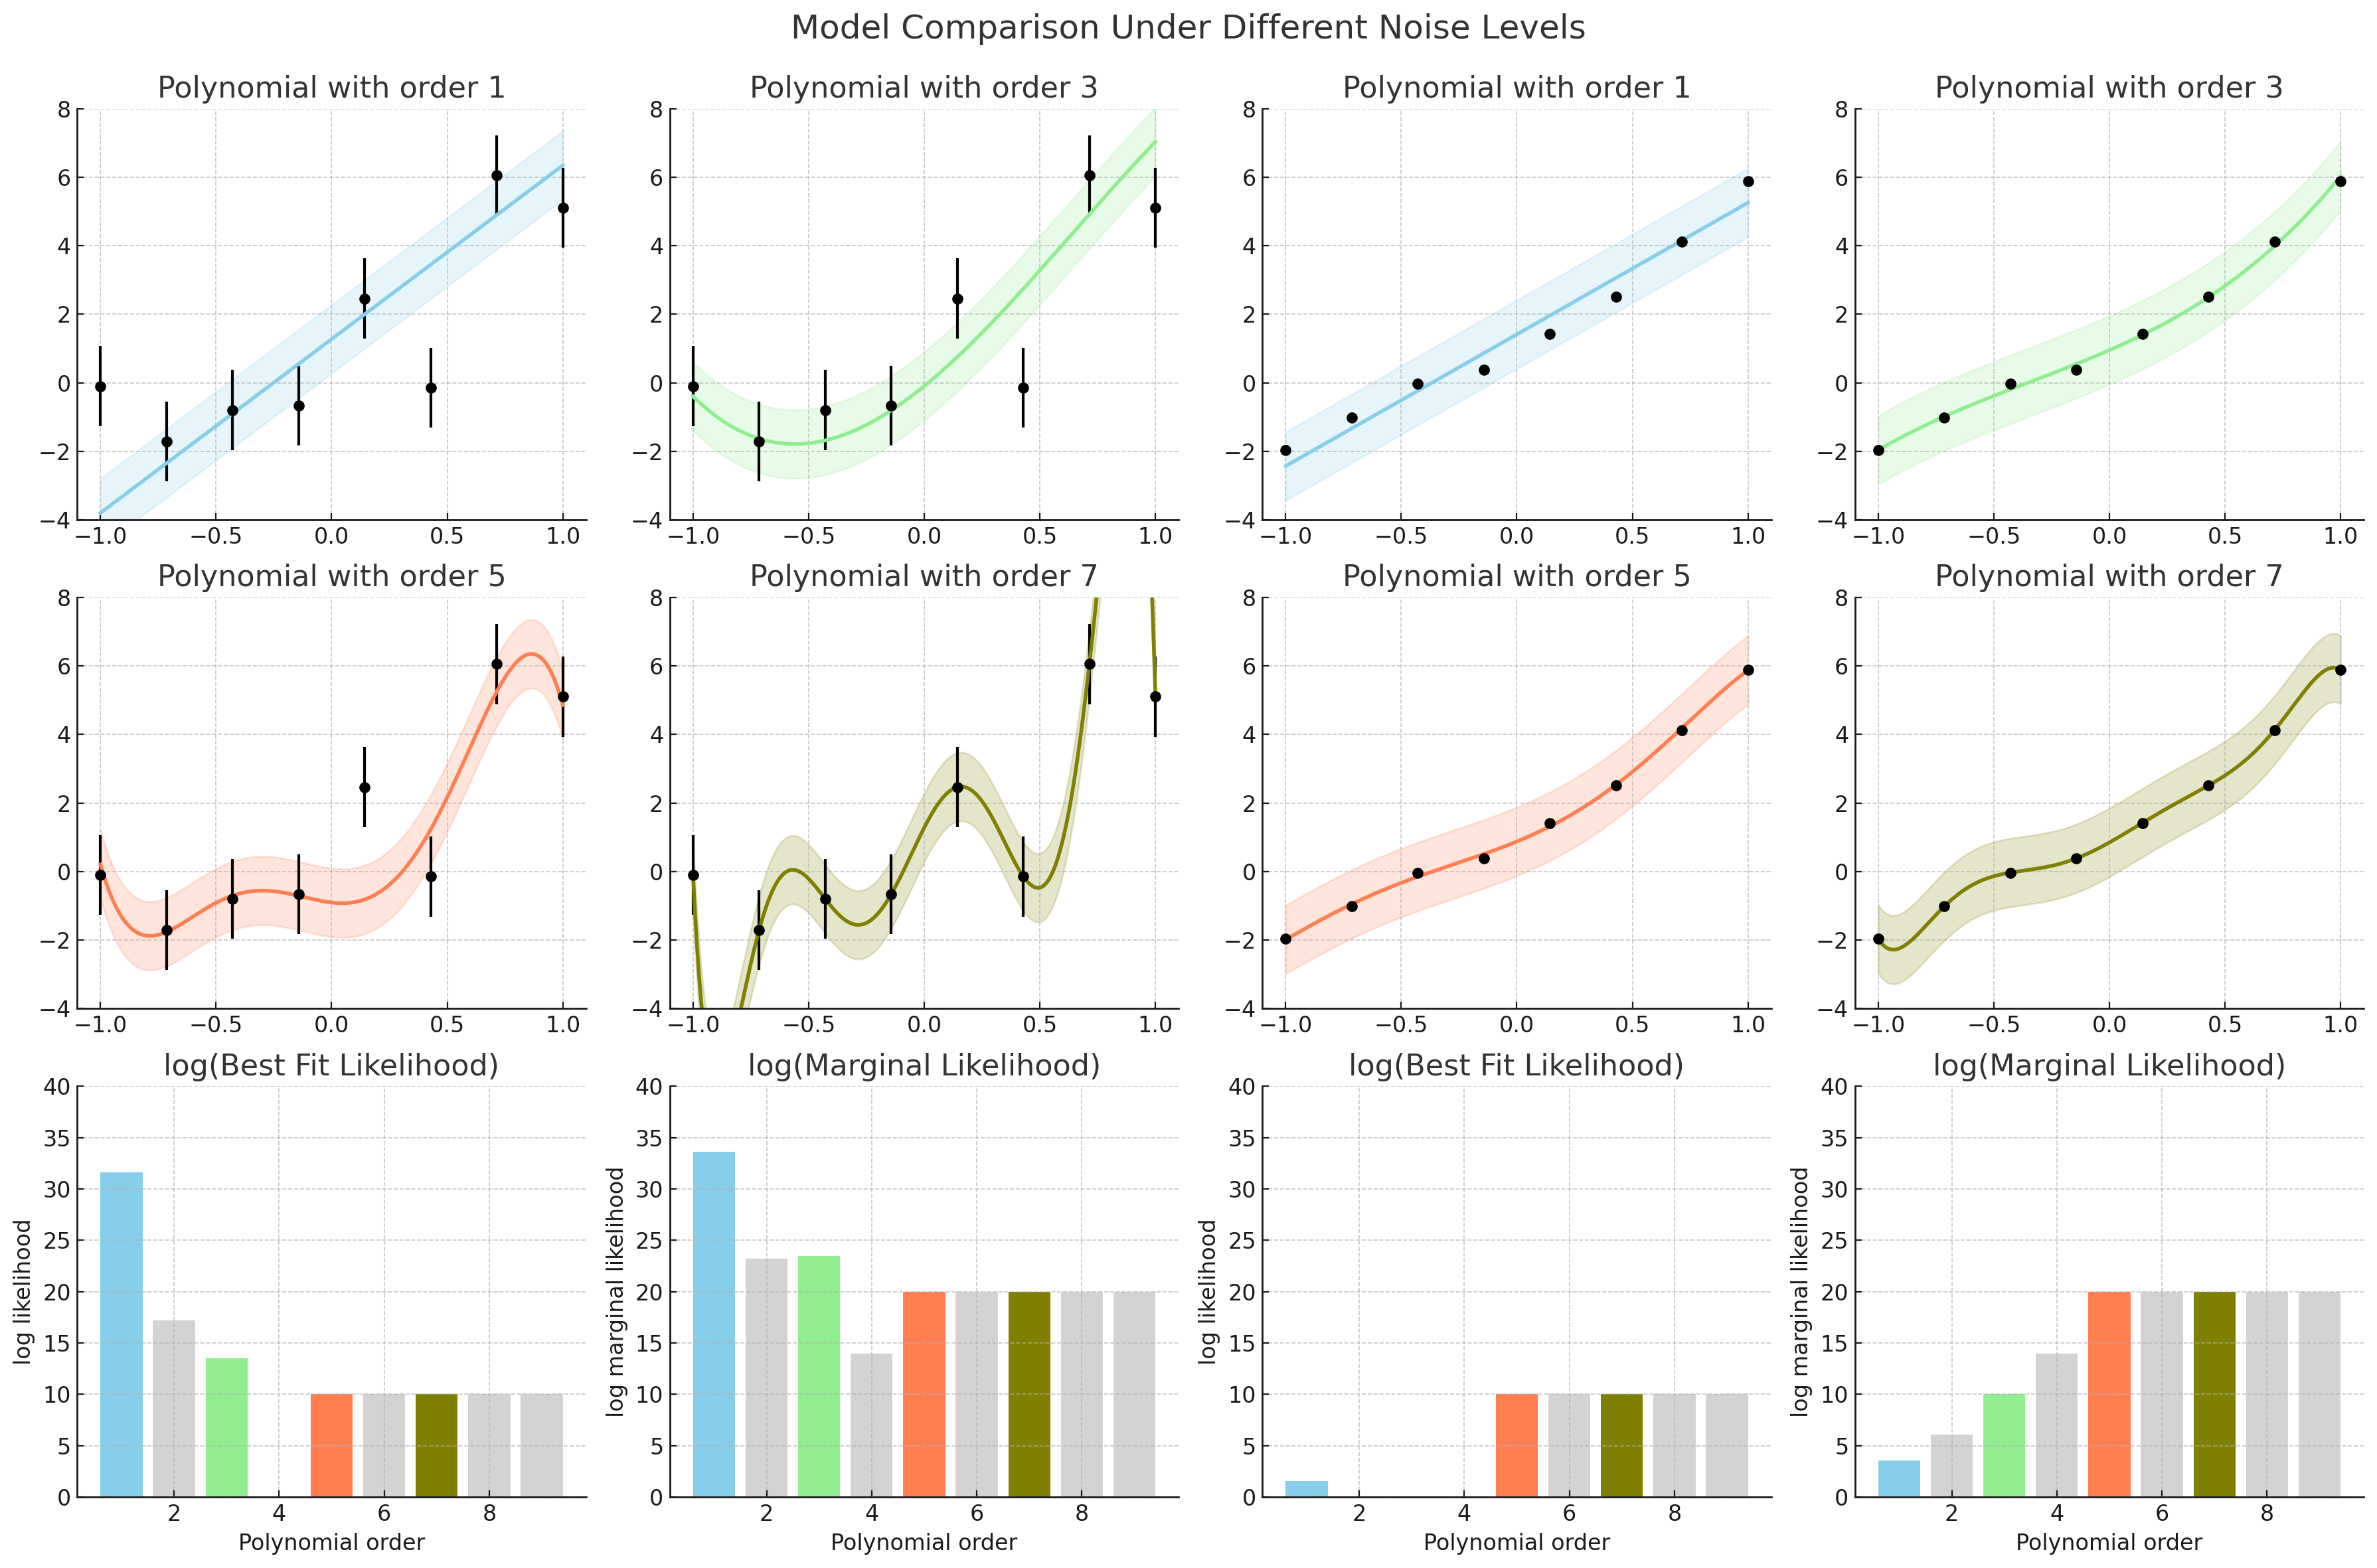
\includegraphics[width=0.9\linewidth]{MSc_Statistics_Research_Report_Template/images/output.png} 
\caption{ODR polynomial fits (orders 1, 3, 5, 7) to eight samples from a cubic ground truth under large (left) and small (right) noise. Bottom panels compare the marginal likelihood of different orders, where higher values indicate better model fit; the penalised score favours simpler models at high noise and selects order 3 at low noise.}
\end{figure}

One way to overcome this challenge is to make use of regression algorithms that account for the EIV.
Unlike ordinary least squares (OLS), which assumes error-free predictors, EIV algorithms explicitly account for measurement errors in both x and y, thereby mitigating attenuation bias in slope estimation \citep{fuller2009, carroll2006}. For nonlinear models, SINDy tries to learn one suitable candidate among EIV algorithms is Orthogonal Distance Regression (ODR).
ODR offer an effective way to explain these uncertainties on both sides of the regression equation \citep{boggs1989}. 
Empirical studies have shown that EIV-type estimators, such as Deming regression, principal component regression, and Bayesian EIV, provide less biased estimates than OLS in the presence of measurement errors \citep{mikkonen2019}. Comparative work has also highlighted the relative advantages of ODR and Bayesian EIV in geometric fitting tasks, such as circle and ellipse fitting, where ODR offers robust nonlinear extensions \citep{splett2018}. More recently, ODR has been incorporated into Bayesian model discovery frameworks, including SINDy, to improve robustness when both states and derivatives are noisy \citep{quade2018, champion2020}. Collectively, these contributions establish EIV and ODR as essential tools for handling measurement error in both predictors and responses across statistical modelling and data-driven scientific discovery.


\subsection{Contribution of this study}


This thesis introduces three novel model methods that can solve the selection of one-dimensional sparse polynomial models with noise. Because we aim to establish and validate the proposed methods in a controlled and transparent setting, so we consider the one-dimensional polynomial model as a simpler archetypal problem.

We develop a Bayesian evidence–based framework for sparse polynomial model selection that directly computes posterior model probabilities, thereby integrating Occam’s razor in a principled way. This approach enables model selection under the noise in the response variable, balancing fit and complexity without relying on asymptotic information criteria such as AIC or BIC. In doing so, it provides a fully probabilistic mechanism for identifying the most parsimonious model structure. 
In addition, we employ the SINDy methodology to mitigate the risk of overfitting in model selection under this setting, further enhancing interpretability and robustness.

To address the more challenging case where both predictors and responses are corrupted by measurement errors, we extend the SINDy framework by incorporating ODR. By coupling ODR with sequential thresholding, the proposed Sequentially Thresholded Least Squares with ODR (STLSQ-ODR) method explicitly corrects for EIV, yielding more robust coefficient estimates and enabling reliable recovery of governing equations under correlated and heavy-tailed noise.

Through simulation studies, we demonstrate the comparative advantages of each method under different noise structures and highlight the potential for future integration of Bayesian evidence with ODR-based sparsification to create a comprehensive noise-robust model selection framework.


\subsection{Structure of the paper}
The rest of this paper is organised as follows. In Section \ref{sec:meth}, we provide a detailed overview of the polynomial regression framework and its role in sparse model discovery. We first review the Bayesian razor method \citep{mackay2003}, which leverages Bayesian evidence and the Occam factor to balance model fit and complexity. This approach is easily applied in cases where noise is present only in the response variable, allowing for model selection among competing polynomial structures. We then introduce the STLSQ framework for model selection with noise in the response variable. Then we introduce the EIV problem that can be dealt with by 0ODR. We then introduce the STLSQ-ODR framework, which integrates sparse thresholded regression with ODR to explicitly account for measurement errors in both predictors and the response variable. Section \ref{sec:simu} presents empirical studies showcasing the performance of these three approaches under different noise structures and correlation settings, including both synthetic data experiments and robustness analyses. In Section \ref{sec:disc}, we compare the strengths and limitations of the three methods. Specifically, we discuss why the Bayesian razor excels in balancing model fit and complexity under moderate response noise, while the STLSQ-ODR method provides more robust estimation in scenarios where measurement errors occur in both inputs and outputs. Finally, we conclude with remarks on potential extensions and future research directions, including the integration of Bayesian evidence with ODR-based sparsification to enable more comprehensive model selection.